\documentclass[a4paper,12pt]{report}
\usepackage[spanish,mexico]{babel}
\usepackage[utf8]{inputenc}
\usepackage[T1]{fontenc}
\usepackage{amsmath}
\usepackage{amssymb}
\usepackage{multirow}
\usepackage{wasysym}
\usepackage[dvipsnames,pdftex]{color}
\usepackage[colorinlistoftodos]{todonotes}
\usepackage[left=3.0cm,right=2.0cm,top=3.0cm,bottom=2cm]{geometry}
%\usepackage{helvet}
%\renewcommand{\familydefault}{\sfdefault}
\setlength{\oddsidemargin}{0in}
\usepackage{float}
 \setlength{\textwidth}{6in}
 \setlength{\topmargin}{0in}
 \setlength{\voffset}{-0.5in}
 \setlength{\hoffset}{0.5in}
 \setlength{\textheight}{9in}
 \setlength{\textwidth}{6in}
 \setlength{\topskip}{0in}
 \setlength{\parskip}{2ex}
 \renewcommand{\baselinestretch}{1}
\usepackage{diagbox}
\usepackage{array}
\usepackage{listings}
\usepackage{caption}
%%% comandos definidos por el usuario

\begin{document}
\setcounter{page}{1}
\pagenumbering{roman}
\thispagestyle{empty}
\begin{center}
{\huge UNIVERSIDAD NACIONAL DE INGENIERÍA}\\[0.9cm]
{\Large FACULTAD DE INGENIERÍA MECÁNICA}\\[0.6in]
\end{center}
\begin{figure}[h]
\begin{center}
\includegraphics[scale=0.2]{LogoUNI}
\vspace{0cm}
\end{center}
\end{figure}
\vspace{0.5cm}
\begin{center}
QUINTO INFORME DE LABORATORIO\\
CIENCIA DE LOS MATERIALES II\\[14mm]
{\Large OXIDACIÓN Y CORROSIÓN}\\[10mm]
\vfill
LIMA - PERÚ \hfill NOVIEMBRE 2018
\end{center}
\newpage
\thispagestyle{empty}
\begin{center}
{\huge OXIDACIÓN Y CORROSIÓN}\\[0.7cm]
\small ENTREGADO:\\[0.3cm]
\small 1 DICIEMBRE 2018\\[0.9cm]
\end{center}
\begin{flushleft}
{\large INTEGRANTES:}\\[3cm]
\end{flushleft}
%\begin{tabular}{c@{\hspace{0.5in}}c}
%\rule[1pt]{2.6in}{1pt}&\rule[1pt]{2.6in}{1pt}\\
%Huaroto Villavicencio Josué, 20174070I & Fuentes Valdivia Martin, 2017\\[1.5cm]
%\rule[1pt]{2.6in}{1pt}&\rule[1pt]{2.6in}{1pt}\\
%Saldivar Montero Perruardo, 2017 & Nombre 3, 2017\\[1cm]
%\rule[1pt]{2.6in}{1pt}&\rule[1pt]{2.6in}{1pt}\\
%Nombre 4, 2017 & Nombre 5, 2017 \\[1.5cm]
\begin{tabular}{c@{\hspace{0.5in}}c}
\rule[1pt]{2.6in}{1pt}&\rule[1pt]{2.6in}{1pt}\\
Huaroto Villavicencio Josué, 20174070I & Landeo Sosa Bruno, 20172024J\\[2.5cm]
\rule[1pt]{2.6in}{1pt}&\rule[1pt]{2.6in}{1pt}\\
Quesquen Vitor Angel, 20170270C & Saldivar Montero Eduardo, 20174013E\\[2.5cm]
\rule[1pt]{2.6in}{1pt}&\rule[1pt]{2.6in}{1pt}\\
Saravia Echevarria Henrry, 20170233K & Sotelo Cavero Sergio, 20172125K \\[1.6cm]
\end{tabular}
%\\[0.7cm]
{\large PROFESOR:} \\[1.15cm]
\begin{center}
\begin{tabular}{c}
\rule[3pt]{4.8in}{1pt}\\[1pt]
ING. LUIS SOSA, JOSE 
\end{tabular}
\end{center}
\vfill
%\newpage
%\begin{center}
%{\Large \bf{RESUMEN}}
%\end{center}
\newpage
\tableofcontents
\listoffigures
\addcontentsline{toc}{chapter}{Índice de Figuras}
\chapter{Objetivos}
\begin{enumerate}
\item Comprobar el efecto que tiene la temperatura sobre la reacción entre la superficie de un metal y el medio ambiente (aire libre).
\item Cuantificar la pérdida que se da en un material por oxidación, tanto perdida másica como volumétrica.
\item Poder predecir el comportamiento de cada material, y así ser capaces de clasificar un material como resistente a la oxidación, y por lo tanto óptimo para un proceso a alta temperatura, o pobremente resistente, por lo cual no se recomendaría su uso.
\end{enumerate}
\pagenumbering{arabic} %%% esto es para regresar el modo de numeración a numeración arábiga
\setcounter{page}{1}  %%% empezamos en página 1
\chapter{Materiales}
\begin{enumerate}
\item Horno eléctrico
\begin{figure}[H]
\begin{center}
\includegraphics[scale=0.6]{horno}
\caption{Horno eléctrico del laboratorio}
\end{center}
\end{figure}
\newpage
\item Probetas de cobre, bronce y acero
\begin{figure}[H]
\begin{center}
\includegraphics[scale=0.7]{prob}
\caption{Probetas de cobre, bronce y acero del laboratorio}
\end{center}
\end{figure}
\item Vernier digital
\begin{figure}[H]
\begin{center}
\includegraphics[scale=0.23]{vdi}
\caption{Vernier digital marca Mitutoyo}
\end{center}
\end{figure}
\item Balanza de laboratorio
\begin{figure}[H]
\begin{center}
\includegraphics[scale=0.4]{balanza}
\caption{Balanza de laboratorio marca Sores modelo ASX}
\end{center}
\end{figure}
\item Lijas
\begin{figure}[H]
\begin{center}
\includegraphics[scale=0.25]{lijar}
\caption{Lijas del laboratorio}
\end{center}
\end{figure}
\end{enumerate}
\chapter{Procedimiento de medida}
\begin{enumerate}
\item Desbastar las probetas para eliminar posibles impurezas que puedan afectar el cálculo de su masa.
\begin{figure}[H]
\begin{center}
\includegraphics[scale=1]{prob}
\caption{Probetas del laboratorio}
\end{center}
\end{figure}
\item Pesar las probetas, medir sus dimensiones y anotar.
\newpage
\item Someter cada probeta a un calentamiento de 850$^{\circ}$C con tiempos de 30, 60, 100 y 120 minutos (probetas 1, 2, 3 y 4, respectivamente). 
\begin{figure}[H]
\begin{center}
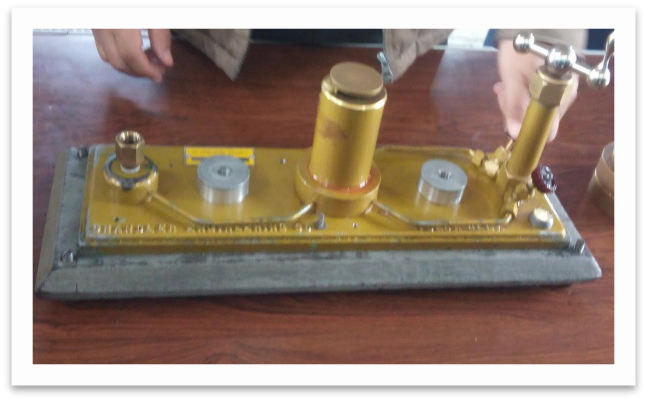
\includegraphics[scale=0.5]{proc2}
\caption{Colocando las probetas en el horno precalentado}
\end{center}
\end{figure}
\begin{figure}[H]
\begin{center}
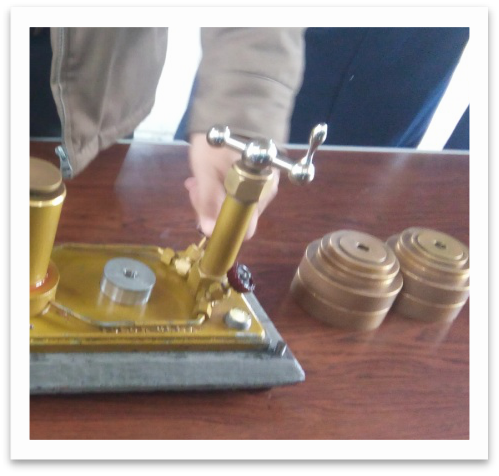
\includegraphics[scale=0.5]{proc3}
\caption{Probetas antes del calentamiento}
\end{center}
\end{figure}
\item Desbastar nuevamente cada probeta hasta eliminar la capa de óxido formada por el tratamiento térmico.
\begin{figure}[H]
\begin{center}
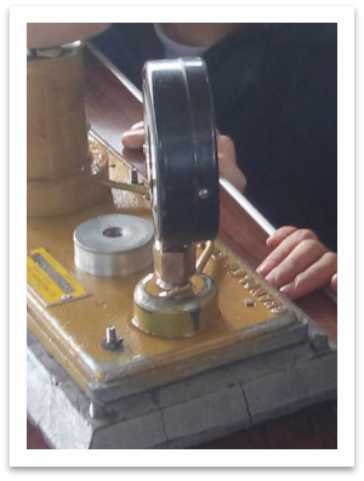
\includegraphics[scale=0.45]{proc4}
\caption{Restos de óxido después del desbaste}
\end{center}
\end{figure}
\item Pesar cada probeta, medir sus nuevas dimensiones y comparar con los resultados anteriores.
\begin{figure}[H]
\begin{center}
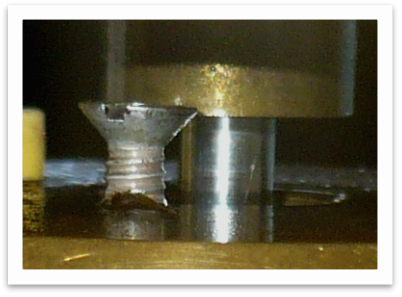
\includegraphics[scale=0.4]{proc5}
\caption{Pesando las probetas}
\end{center}
\end{figure}
\end{enumerate}
\chapter{Cálculos y resultados}
Temperatura del horno = 850$^{\circ}$C.\\
El ensayo comienza a las 9:30.
\begin{figure}[H]
\begin{center}
\includegraphics[scale=0.65]{calculos1}
\end{center}
\end{figure}
\newpage
Hallamos el volumen antes del ensayo, la densidad y la diferencia de masa:
\begin{figure}[H]
\begin{center}
\includegraphics[scale=0.7]{calculos2}
\end{center}
\end{figure}
Con los datos anteriores se calcula el espesor perdido, asumimos que la capa de óxido se forma en mayor cantidad sobre el contorno del cilindro y no sobre las caras. Con esta suposición se tiene la siguiente expresión:
$$
\Delta\mathrm{Vol} = V_{i} - \frac{\pi \cdot h\cdot (D-2e)^{2}}{4}
$$
$$
\rho = \frac{\Delta \mathrm{m}}{\Delta \mathrm{V}}
$$
Usando estas 2 fórmulas se obtiene una expresión para calcular el espesor aproximado:
$$
2e = D - \sqrt{\frac{4 \cdot \left( V_{i}-\frac{\Delta \mathrm{m}}{\rho} \right)}{\pi \cdot h}}
$$
\begin{figure}[H]
\begin{center}
\includegraphics[scale=0.7]{calculos3}
\end{center}
\end{figure}
Con estos datos se puede graficar el espesor en función del tiempo:
\begin{figure}[H]
\begin{center}
\includegraphics[scale=0.7]{calculos4}
\end{center}
\end{figure}
\begin{figure}[H]
\begin{center}
\includegraphics[scale=0.7]{calculos5}
\end{center}
\end{figure}
\begin{figure}[H]
\begin{center}
\includegraphics[scale=0.7]{calculos6}
\end{center}
\end{figure}
\chapter{Conclusiones y recomendaciones}
\begin{enumerate}
\item La corrosión causa una destrucción lenta y progresiva, a partir de la superficie, de un metal por la acción de un agente exterior.
\item Para que se realice la corrosión necesariamente deben existir las condiciones necesarias: Un ambiente húmedo ácido o básico, elementos oxidantes y reductores que actúen como cátodo y ánodo-cierta concentración de sales o elementos inertes que actúen como puente salino.
\item La velocidad de ataque se incrementa sustancialmente con la temperatura a la que se someten las probetas.
\item El espesor perdido por oxidación de las probetas varía directamente proporcional al tiempo en el que estas están en el horno.
\item La cantidad producida de óxido depende del material del que están hechos cada probeta.
\item La corrosión provoca significativas pérdidas de material lo que conlleva a pérdidas económicas importantes.
%\item Tu megazord no te hará caso Henrry.
\end{enumerate}
\chapter{Anexos}
\section*{Cuestionario}
\begin{enumerate}
\item \textbf{¿En qué casos la oxidación presenta un comportamiento de tipo lineal?} \\
En los casos donde el volumen del óxido es inferior al del metal pues no habrá una capa decisiva que impida la linealidad en la formación del óxido a lo largo del tiempo; por tanto, la relación del volumen específico del óxido al del metal es inferior a uno, además la capa de óxido es discontinua haciendo que el oxígeno la atraviese fácilmente y continúa atacando al mental. Los metales que presentan esta condición son los ligeros, alcalinos térreos y las tierras raras.\\
Ley lineal:
$$
W = K_{L}\cdot t
$$
\item \textbf{El hierro por encima de los 500$^{\circ}$C presenta un oxido complejo, debido a sus varias valencias. Sabiendo que se forman los óxidos: FeO, Fe$_{2}$O$_{3}$ y Fe$_{3}$O$_{4}$, indicar esquemáticamente sus ubicaciones en una capa de oxido.}\\
A altas temperaturas los tres tipos de óxido de hierro estables se forman en capas paralelas en función de la cantidad de oxígeno. La capa interior corresponde a la wustita (FeO), la cual es la de menor contenido de oxígeno (23.7\% 0 en peso), la capa intermedia corresponde a la magnetita (Fe$_{3}$O$_{4}$) que tiene 27.72\% 0 en peso, y la capa exterior corresponde a la hematita (Fe$_{2}$O$_{3}$), que es la de mayor contenido de oxígeno (30.6\% 0).
\item \textbf{Un cilindro metálico sólido con un diámetro inicial de 12.65$\,$mm, una altura de 18.58$\,$mm y una masa inicial de 20.5798 gramos es introducido en un horno a 850$^{\circ}$C durante tres horas. Su masa final es de 19.6932 gramos. Determinar el espesor del material perdido por oxidación.}\\
Datos:
\begin{itemize}
\item D=12.65$\,$mm
\item h=18.58$\,$mm
\item m=20.5798$\,$g
\item D'=12.65-2$\cdot$e$\,$mm
\item h'=18.58-2$\cdot$e$\,$mm
\item m'=19.6932$\,$g
\end{itemize}
$$
\frac{m}{\frac{\pi D^{2}}{4} h} = \frac{m'}{\frac{\pi D'^{2}}{4} h'} 
$$
$$
\frac{20.5798}{12.65^{2} \cdot 18.58} = \frac{19.6932}{(12.65-2\cdot e)^{2} \cdot (18.58-2\cdot e)} 
$$
$$
(12.65-2\cdot e)^{2}(18.58-2\cdot e) = 2845.129 \longrightarrow e=0.1031
$$
\item \textbf{Un deposito abierto de acero que contiene un electrolito corrosivo sufre una perdida de material de 2 g/m$^{2}$ por día. Calcule la perdida expresada en mdd. 1 mdd = 1 miligramo/decímetro cuadrado por día. Calcule el sobre espesor  de las paredes y fondo de dicho deposito para que dure sin perforarse al menos 10 años. Considerar la densidad del acero 7,87 gr/cm$^{3}$.}\\
Primero calculamos la perdida en md.
$$
2\cdot \frac{\mathrm{g}}{\mathrm{m^{2}} \, \mathrm{dia}} \cdot \frac{1000 \mathrm{mg}}{1 \mathrm{g}} \cdot \frac{10^{-2} \mathrm{m}^{2}}{1 \mathrm{dm}^{2}} = 20 \mathrm{md}
$$
Ahora calculamos la perdida por cada metro cuadrado y en 10 años, también calculamos el volumen de la perdida y finalmente el espesor.
$$
20 \cdot \frac{\mathrm{mg}}{\mathrm{dm^{2}} \, \mathrm{dia}} \cdot \frac{1 \mathrm{kg}}{10^{6} \mathrm{mg}} \cdot \frac{100 \mathrm{dm}^{2}}{1 \mathrm{m}^{2}} \cdot \frac{365 \mathrm{dias}}{1 \text{año}} = 0.73 \frac{\mathrm{kg}}{\mathrm{m}^{2} \, \text{año}} \xrightarrow{\text{10 años después}} 7.3 \frac{\mathrm{kg}}{\mathrm{m}^{2}}
$$
$$
V=\frac{7.3 \text{kg}}{7.87\cdot 10^{3} \text{kg}/\mathrm{m}^{3}} = 0.9276 \cdot 10^{-3} \mathrm{m}^{3} \Longrightarrow e=\frac{V}{\mathrm{Area}} = 0.92757  \, \mathrm{mm}
$$
\item \textbf{Se quiere utilizar un determinado tipo de acero para la fabricación de tanques que almacenaran un líquido corrosivo. Para ello se expusieron probetas de este acero a la acción de este liquido corrosivo y se observo una perdida media de 30 miligramos/decímetro cuadrado por día.  Determinar si el acero seleccionado es el adecuado. Un material se considera bastante resistente y puede utilizarse si su velocidad de corrosión  es menor o igual a 1 mm/año.}\\
Primero se calcula la pérdida de masa en un año, para esto se hace un cambio de unidades:
$$
\frac{30 \mathrm{mg}}{\mathrm{dm}^{2}\mathrm{dia}} \cdot \frac{1\mathrm{g}}{1000\mathrm{mg}}\cdot \frac{365 \mathrm{dias}}{1 \mathrm{a\text{ñ}o}} \cdot \frac{100 \mathrm{dm}^{2}}{1 \mathrm{m}^{2}} = 1.09 \frac{\mathrm{kg}}{\text{año}}
$$
Para un año se tiene una masa perdida de 1.09 kg. El volumen de esta masa es:
$$
V=\frac{1.09 \mathrm{kg}}{7.87 \mathrm{kg/m^{3}}} = 1.38\cdot 10^{-4} \, m^{3}
$$
Ahora se calcula el espesor perdido:
$$
V=A\cdot e
$$
Para un metro cuadrado del tanque:
$$
e=0.138 \mathrm{mm/\text{año}}
$$
Según tablas, como el espesor es menor que 1 mm por año, se deduce que el acero elegido es muy resistente al ataque corrosivo del liquido que almacenara.
\end{enumerate}
\begin{thebibliography}{99}  %%%este es un contador para el número de bibliografías utilizados.
\addcontentsline{toc}{chapter}{Bibliograf\'{\i}a} %%% Para introducir la bibliografía en el índice.
%\bibitem{Rahman}{Rahman,Aminur y Doe, Hidekazu; ``Ion transfer of tetraalkylammonium cations at an interface between 
%frozen aqueous solution and 1,2-dichloroethane".{\em{Journal of Electroanalytical Chemistry}} {\bfseries 424},159,(1997).}
%\bibitem{Martins}{Martins, M.C., Pereira, C.M., Girault,H.H y Silva, F.; ``Specific adsorption of tetraalkylammonium 
%cations on the 1,2-dichloroethane/water interface".{\em{Electrochimica Acta}} {\bfseries 50},135,(2004).}
%\bibitem{Ding}{Ding, Zhifeng. ``Spectroelectrochemistry and photoelectrochemistry of charge transfer at liquid/liquid
%interfaces". {\em {Tesis, EPFL,}}(1999).}
%\bibitem{IR}{Princeton Applied Research. \em{Technical Note 101}}
%\bibitem{Beni}{Beni V., Ghita M. y Arrigan D. ``Cyclic and pulse voltammetric study of dopamine at the interface between
%two inmiscible electrolyte solutions". {\em{Biosensors \& Biolectronics}} {\bfseries 20}, 2097, (2005).}
%\bibitem{Samec2}{Samec Z., Lhotsky A., Jänchenová H., y Marecek, V. ``Interfacial tension and impedance measurements
%of interfaces between two inmiscible electrolyte solutions". {\em{Journal of Electroanalytical Chemistry}} {\bfseries
%43}, 47, (2000).}
%\bibitem{Day}{Day R.A. y Underwood A.L. {\textit{Química Analítica Cuantitativa}},5ºed. Prentice-Hall, México, 1998.45-48.}
\bibitem{Keyser}{Zavaleta Gutierrez, Nilthon. ``Corrosión''. {\em{CONCYTEC.}}}
\bibitem{Zolotorevski}{Zolotorevski, V. ``Pruebas Mecánicas y Propiedades de los Metales''.{\em{Editorial MIR.}}}
\bibitem{Lasheras}{Lasheras. ``Tecnología de los Materiales Industriales''.} 
%\bibitem{Dieter}{Dieter. ``Metalurgia mecánica''.}
\bibitem{Apraiz}{Groysman, A. ``Corrosion for everybody''.}
\bibitem{Smith}{Smith, William F. y Ph.D. Hashemi, Javad ``Ciencia e ingeniería de materiales". {\em{
Madrid: McGraw-Hill, Interamericana de España.}} 570, (2004).} 
\bibitem{Callister}{Callister, William D. y Rethwisch, David G. ``Introducción a la ingeniería de los materiales''. {\em{Barcelona Reverté.}}, 960, (2007).} 
\bibitem{Askeland}{Askeland, Donald R., Pradeep P. Phulé y Wright, Wendelin J. ``Ciencia e ingeniería de los materiales''.{\em{México, D.F. Internacional Thomson Editores.}} {\textit{$6^{ta}$ edición}}, 1004, (2012).}
%\bibitem{HARDBANDING}{Tabla de conversión de escala de durezas. \begin{verbatim}http://%hardbandingsolutions.com/postle_sp/hardness.php
%\end{verbatim}}
\end{thebibliography}
\end{document}
